%!TEX program = xelatex
\documentclass[10pt, compress]{beamer}
\usepackage{array}
\usepackage{listings} % for code snippets
\usepackage{enumitem}
\usepackage{xltxtra}
\usepackage{xgreek}
\usepackage{multicol}
\usepackage{commath}
\usepackage{amsmath}
\usepackage[export]{adjustbox}
\usepackage{wrapfig}

\usepackage{subfig}
\renewcommand{\thesubfigure}{\roman{subfigure}}

% matlab
\usepackage{listings}
\usepackage{color} %red, green, blue, yellow, cyan, magenta, black, white
\definecolor{mygreen}{RGB}{28,172,0} % color values Red, Green, Blue
\definecolor{mylilas}{RGB}{170,55,241}
\setbeamercolor{background canvas}{bg=white}

% -------

\usefonttheme{serif} % this made greek work
\setmainfont[Mapping=tex-text]{Liberation Serif}
\usetheme{metropolis}


\begin{document}

\begin{frame}
\thispagestyle{empty}

\begin{flushleft}
% \begin{figure}
%   
\includegraphics[width=.6\linewidth, left]{imgs/square-official-800}
% \end{figure}
\end{flushleft}
\Large{\textbf{Deep Learning Workshop}} \\
% \vspace*{-.05cm}

% \fontsize{10pt}{Εργαστήριο 1 \\ Εισαγωγή στα Σήματα \& Συστήματα με Matlab}
% {\fontsize{12}{40} \selectfont ``A.I. is the new electricity"} \\
% {\fontsize{9}{40} \selectfont \qquad \qquad \qquad \qquad \qquad -Andrew NG} \\
\begin{multicols}{2}
{\fontsize{10}{40} \selectfont ``...what we want is a machine} \\
\vspace*{-.3cm}
{\fontsize{10}{40} \selectfont that can learn from experience."} \\
\vspace*{-.3cm}
{\fontsize{8}{40} \selectfont  \qquad \qquad \qquad \qquad Alan Turing, 1947} \\
% \hrulefill \\

\columnbreak
\vspace*{-1.4cm}

\begin{figure}
  
\includegraphics[width=.4\linewidth, right]{imgs/square-official-800}
\end{figure}
\end{multicols}
\vspace{-1.1cm}
\hrulefill \\
{\fontsize{10}{40} \selectfont Xenofon Karagiannis} \\

% \vspace*{.5cm}
% \begin{figure}
%   \includegraphics[width=.6\linewidth]{imgs/logo-fixed-1}
% \end{figure}
\end{frame}

\setcounter{framenumber}{0}

\begin{frame}
  AI vs ML vs DL vs Data Science \\
  aaaaall hype buzzwords \\

  AI - ANI and AGI (terminator/skynet)
\end{frame}

\begin{frame}
  ``AI is the new electricity". ~Andrew NG \\

  papers and articles!!! \\

  Μερικές εφαρμογές \\
  coursera: google cat,  \\
  edX: , speech reenactment, automatic handwriting gen \\
  other:  medical-images, smart-crops, sefl-driving cars \\

  TensorFlow: an ML platform for solving impactful and challenging problems [\href{https://www.youtube.com/watch?v=NlpS-DhayQA}{link}] \\
  \textbf{Color Restoration} \\
  Let there be Color! [\href{http://iizuka.cs.tsukuba.ac.jp/projects/colorization/extra.html}{link}] \\
  Let there be Color! [\href{https://github.com/satoshiiizuka/siggraph2016_colorization}{github}]
\end{frame}

\begin{frame}
AI failes!\\
\#alexafails \\
cat is dog \\
paypal - got scammed - great

\end{frame}

\begin{frame}
\begin{figure}
  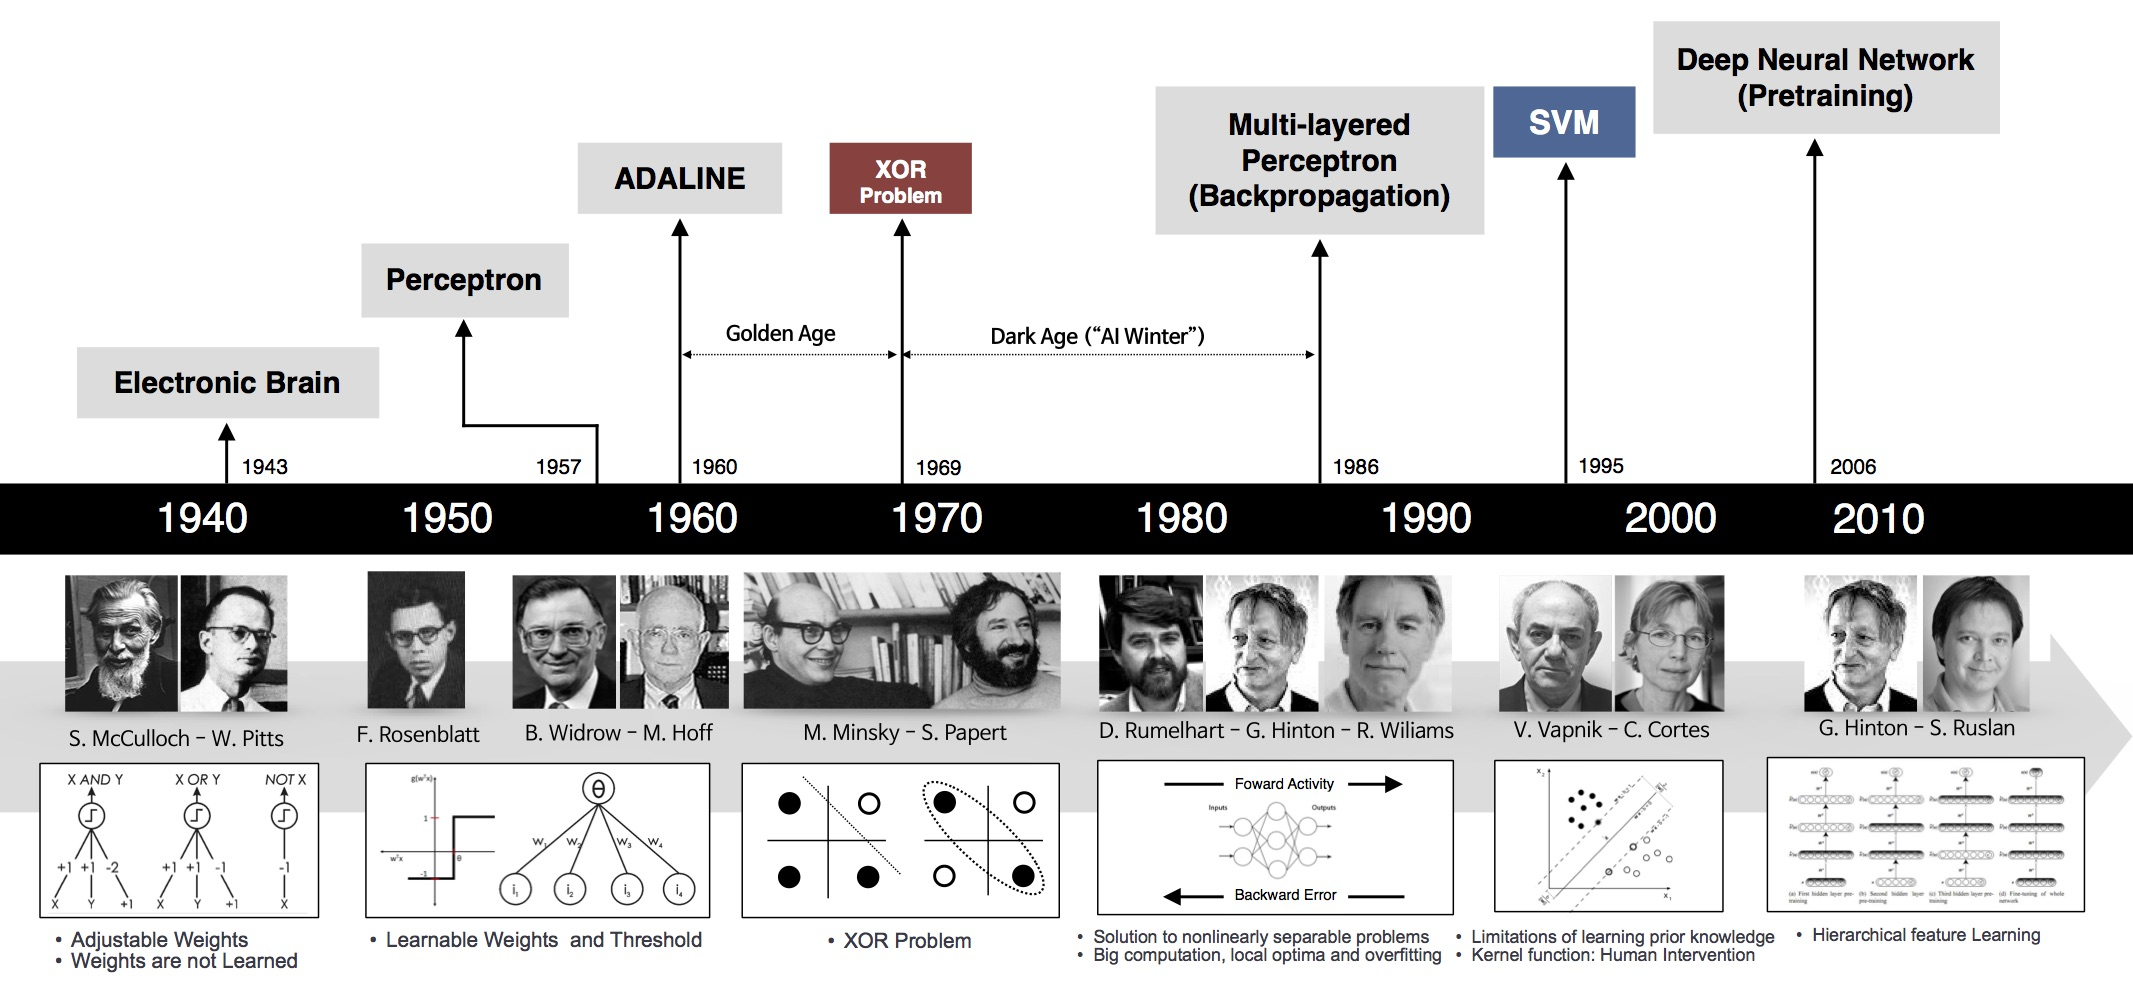
\includegraphics[width=1\linewidth]{imgs/nn_timeline}
\end{figure}
\end{frame}

\begin{frame}
  \vspace*{1cm}
  \textbf{Neuron:} The basic computational unit of the brain  \\
  \textbf{Walter Pitts and Warren McCulloch [1943]:}\\
  \textbf{Thresholded logic unit} (designed to mimic the way a neuron was thought to work) \\
  adjustable but \textit{not learned} weights \\
  \vspace*{-.5cm}
  \begin{eqnarray}
  \mbox{output} & = & \left\{ \begin{array}{ll}
  0 & \mbox{if } \sum_j w_j x_j \leq \mbox{ threshold} \\
  1 & \mbox{if } \sum_j w_j x_j > \mbox{ threshold}
  \end{array} \right.
  \nonumber
  \end{eqnarray}
  \hrulefill \\
  \begin{figure}[ht]
  	\centering
  	\subfloat[Βιολογικός νευρώνας]{%
  		\label{fig:first}%
  		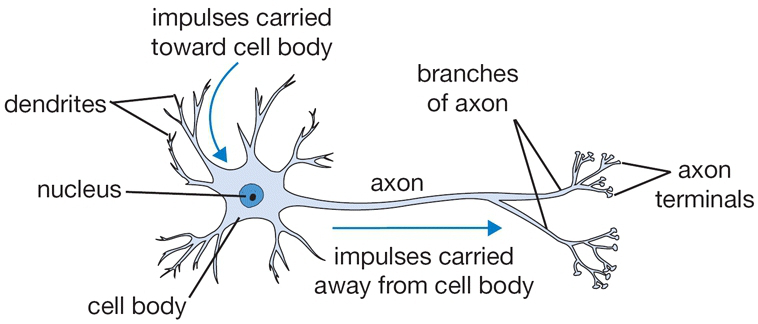
\includegraphics[width=0.5\linewidth]{imgs/neuron}}%
  	\qquad
  	\subfloat[Μαθηματικό μοντέλο - τεχνητός νευρώνας]{%
  		\label{fig:second}%
  		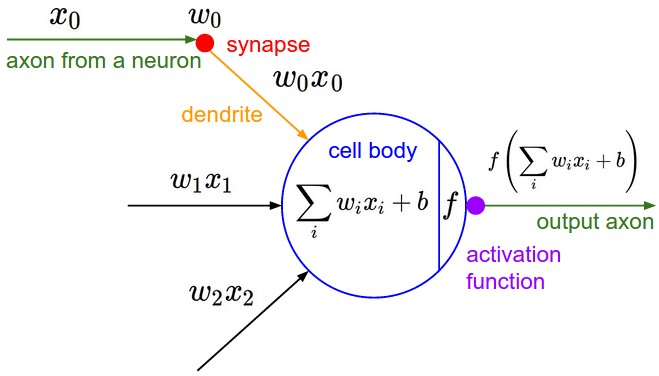
\includegraphics[width=0.4\linewidth]{imgs/artificial_neuron}}
  \end{figure}
\end{frame}

\begin{frame}
  \vspace*{1cm}
  \textbf{Thresholded logic unit}
  % \begin{multicols}{2}
    \begin{eqnarray}
    \mbox{output} & = & \left\{ \begin{array}{ll}
    0 & \mbox{if } \sum_j w_j x_j \leq \mbox{ threshold} \\
    1 & \mbox{if } \sum_j w_j x_j > \mbox{ threshold}
    \end{array} \right.
    \nonumber
    \end{eqnarray}

    % \columnbreak

    \begin{figure}
      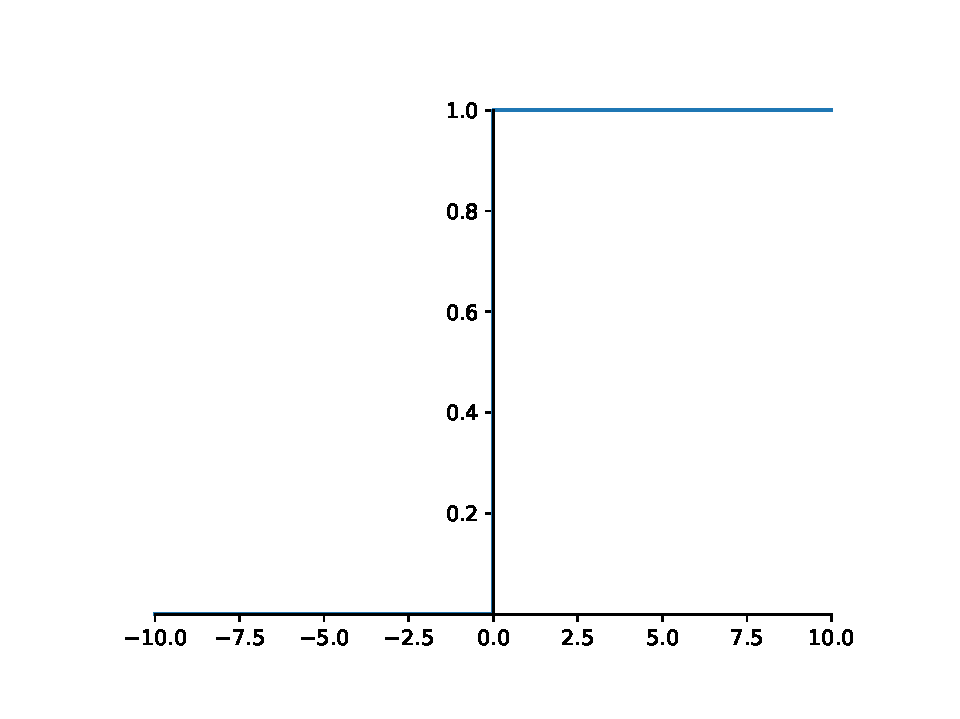
\includegraphics[width=.7\linewidth]{imgs/step.pdf}
    \end{figure}
  % \end{multicols}
\end{frame}

\begin{frame}
  \textbf{Frank Rosenblatt’s “perceptron” [1957]:} \\First real precursor to modern neural networks \\
  Developed \textbf{rule for learning weights}

  \vspace{-.5cm}
  \begin{figure}
    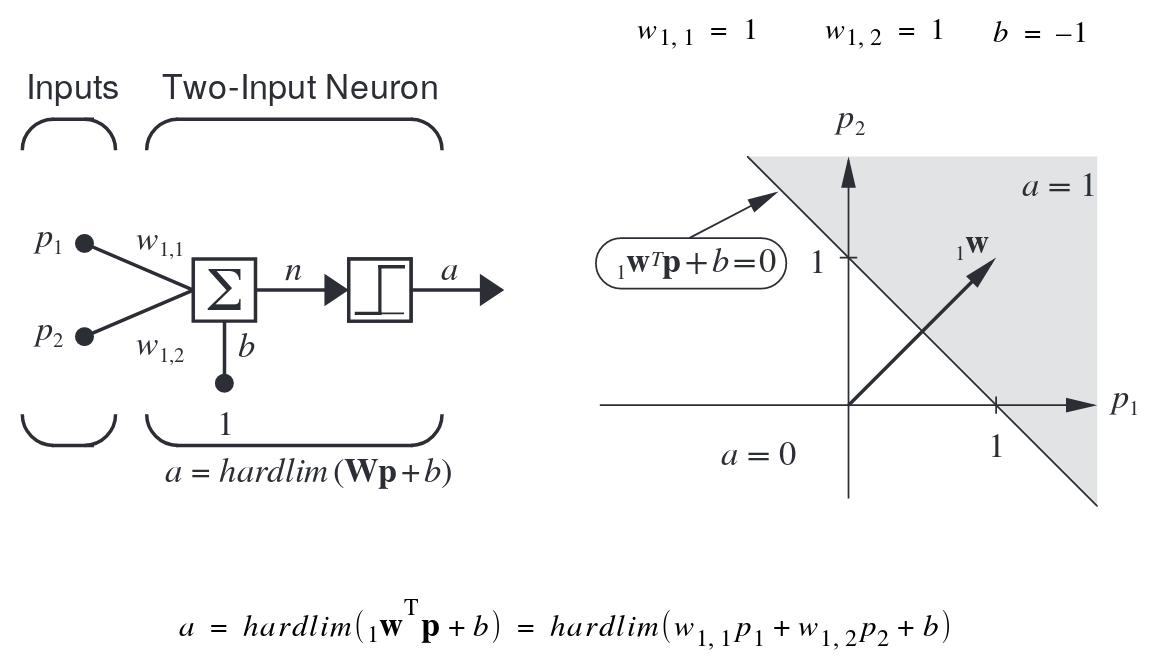
\includegraphics[width=.8\linewidth]{imgs/perceptron_1}
  \end{figure}
  \vspace{-.5cm}
  \textbf{Decision Boundary:} $w_{1,1}p_1 + w_{1,2}p_2 + b = 0$ \\
  \textbf{Linear equation:} $ax + by + c = 0$
\end{frame}

\begin{frame}
  \vspace{1cm}
  \textbf{Supervised Learning} \\
  Network is provided with a set of examples of proper network behavior (inputs/targets)
  $$\{p_1, t_1\}, \{p_2, t_2\}, ..., \{p_Q, t_Q\}$$

  \textbf{Example - OR gate} \\ \hfill \break
  \vspace{-.6cm}
  \begin{figure}
    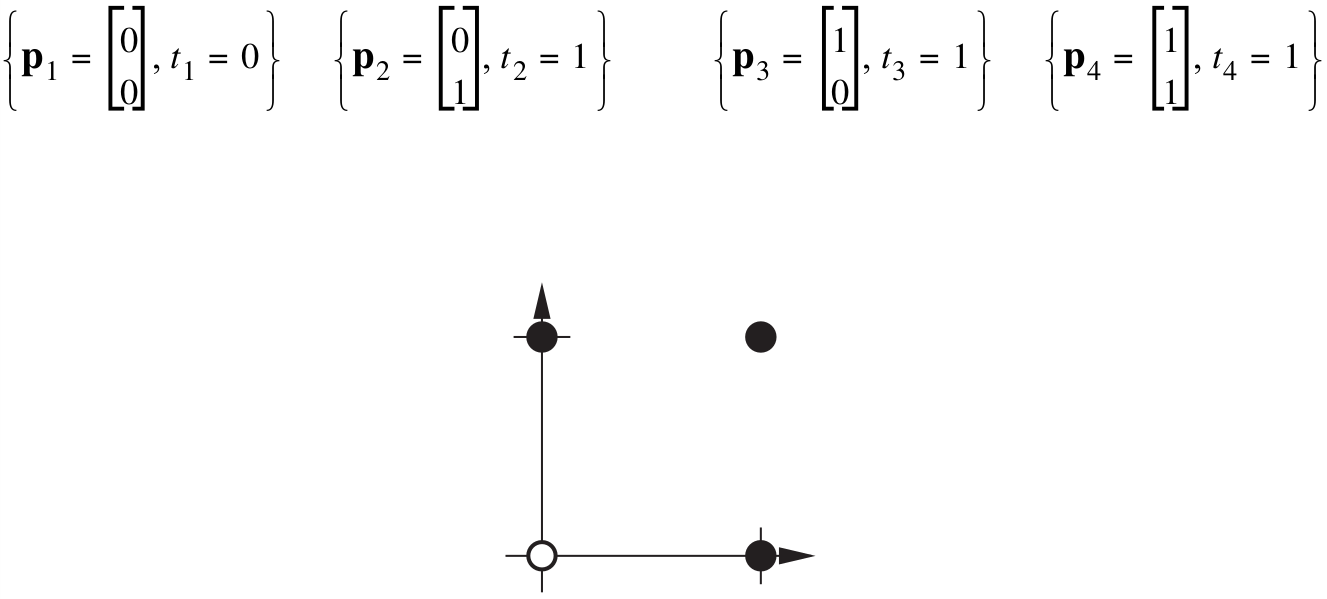
\includegraphics[width=.9\linewidth]{imgs/perceptron_or}
  \end{figure}
\end{frame}

\begin{frame}
  \vspace{1cm}
  \textbf{Example - OR gate}
  \begin{figure}
    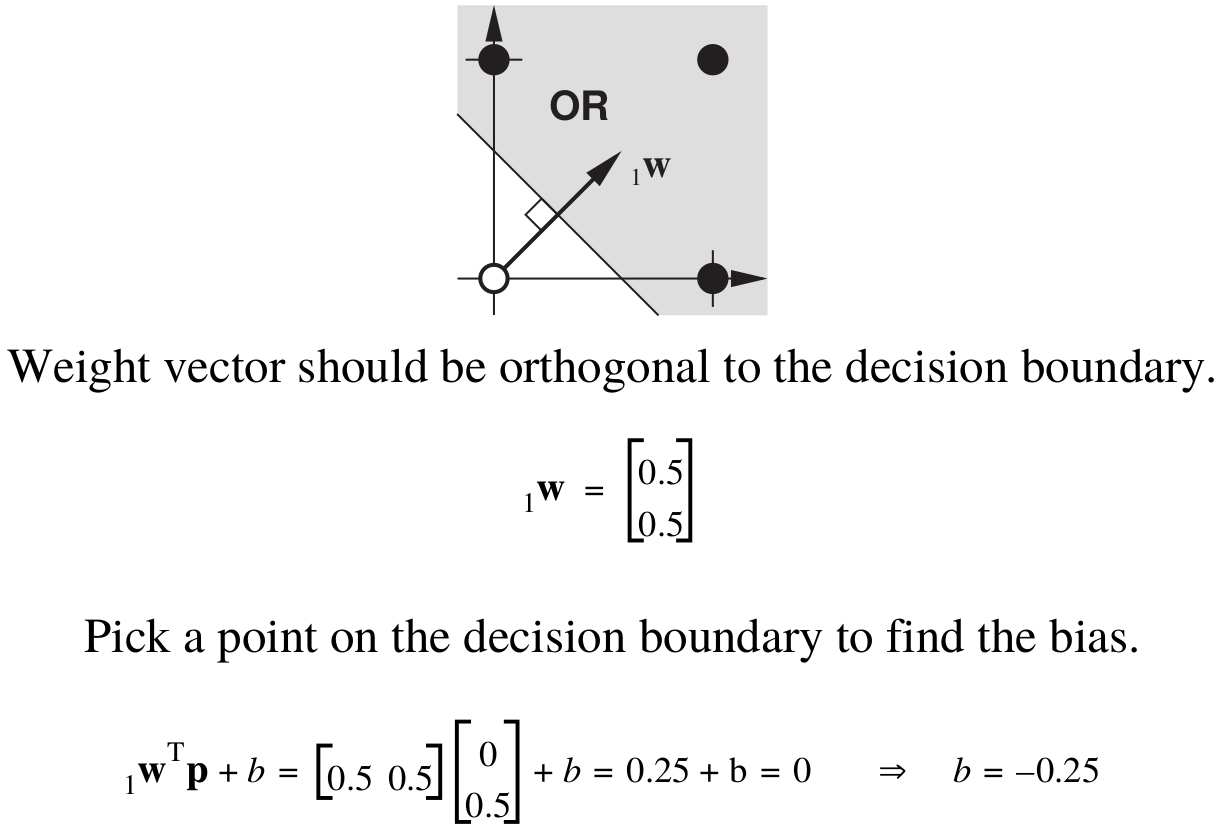
\includegraphics[width=.9\linewidth]{imgs/perceptron_or_2}
  \end{figure}
\end{frame}


\begin{frame}
  \vspace{1cm}
  \textbf{Learning Rule Test Problem}
  \begin{figure}
    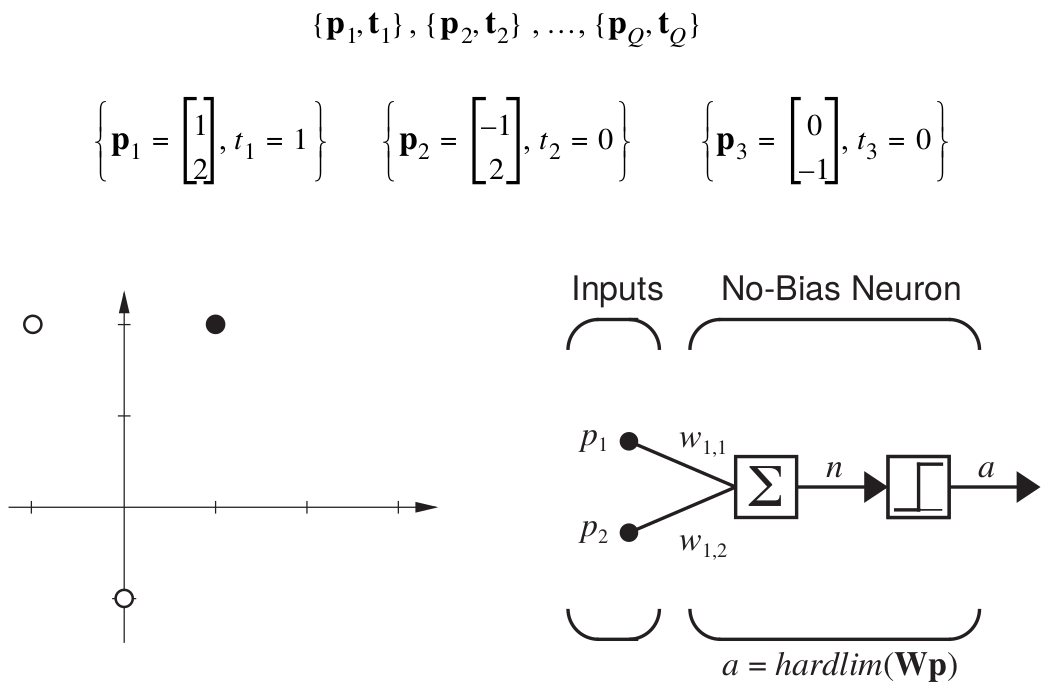
\includegraphics[width=.9\linewidth]{imgs/perceptron_ex_1}
  \end{figure}
\end{frame}

\begin{frame}
  \vspace{1cm}
  \textbf{Starting Point}
  \begin{figure}
    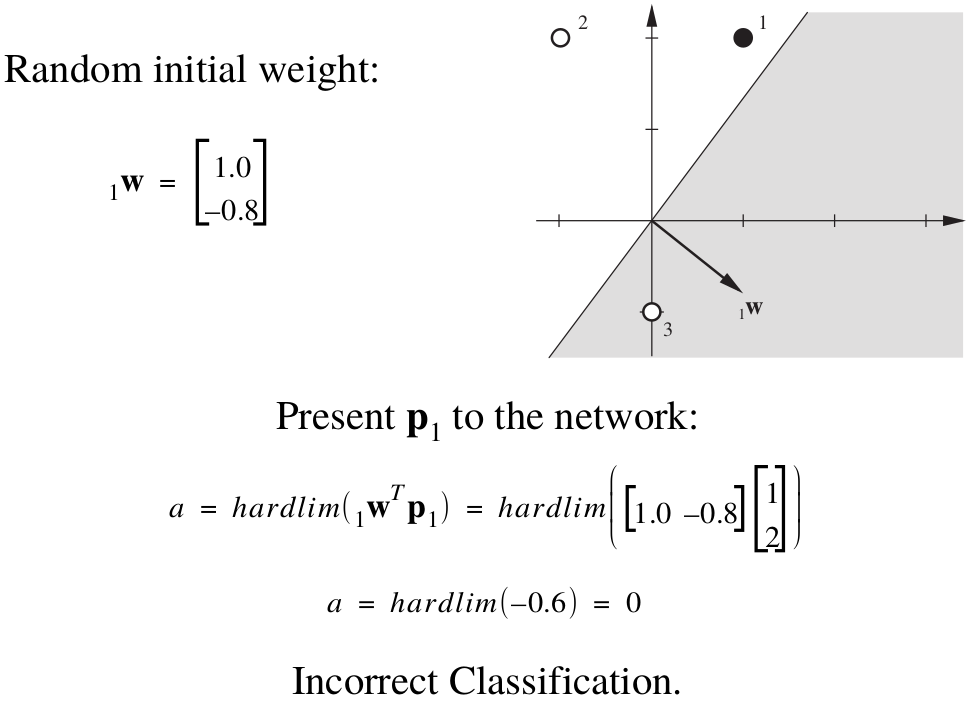
\includegraphics[width=.9\linewidth]{imgs/perceptron_ex_2}
  \end{figure}
\end{frame}

\begin{frame}
  \vspace{1cm}
  \textbf{Tentative Learning Rule}
  \begin{figure}
    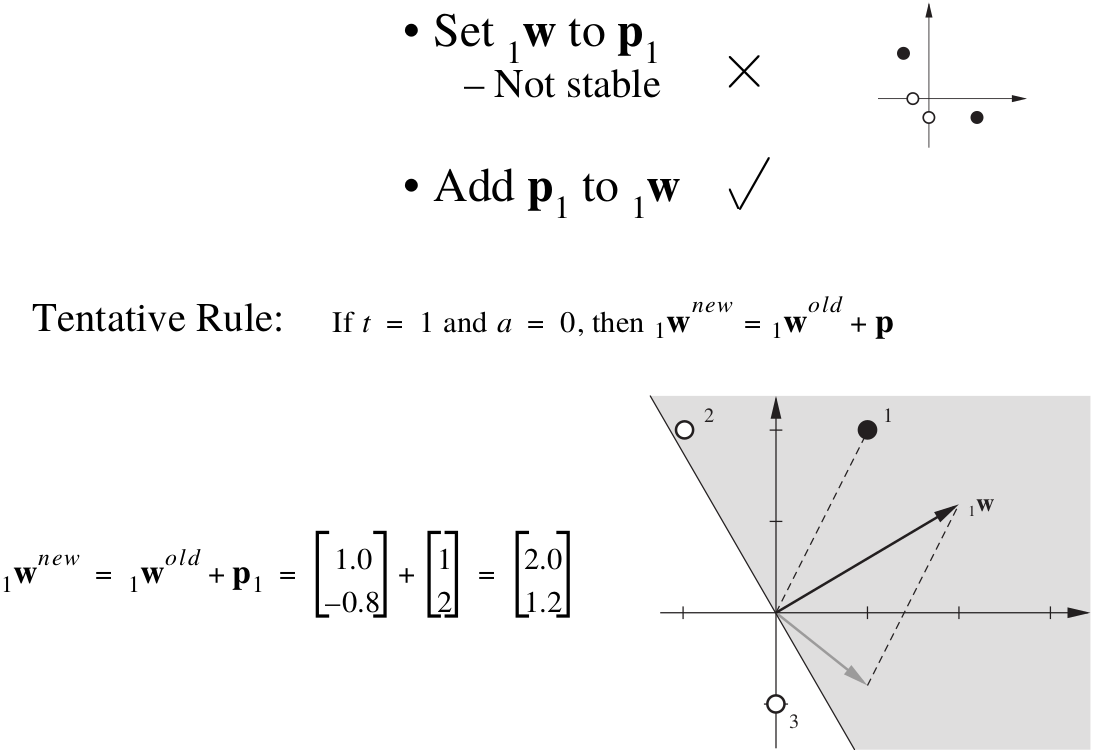
\includegraphics[width=.9\linewidth]{imgs/perceptron_ex_3}
  \end{figure}
\end{frame}

\begin{frame}
  \vspace{1cm}
  \textbf{Second Input Vector}
  \begin{figure}
    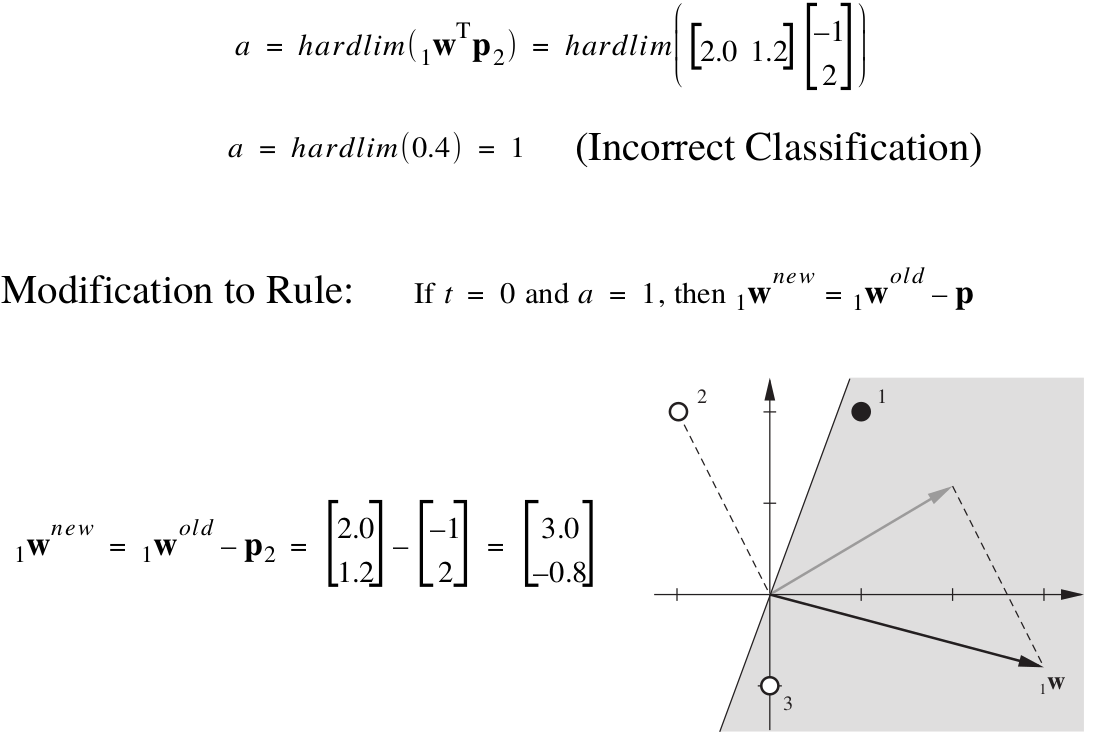
\includegraphics[width=.9\linewidth]{imgs/perceptron_ex_4}
  \end{figure}
\end{frame}

\begin{frame}
  \vspace{1cm}
  \textbf{Third Input Vector}
  \begin{figure}
    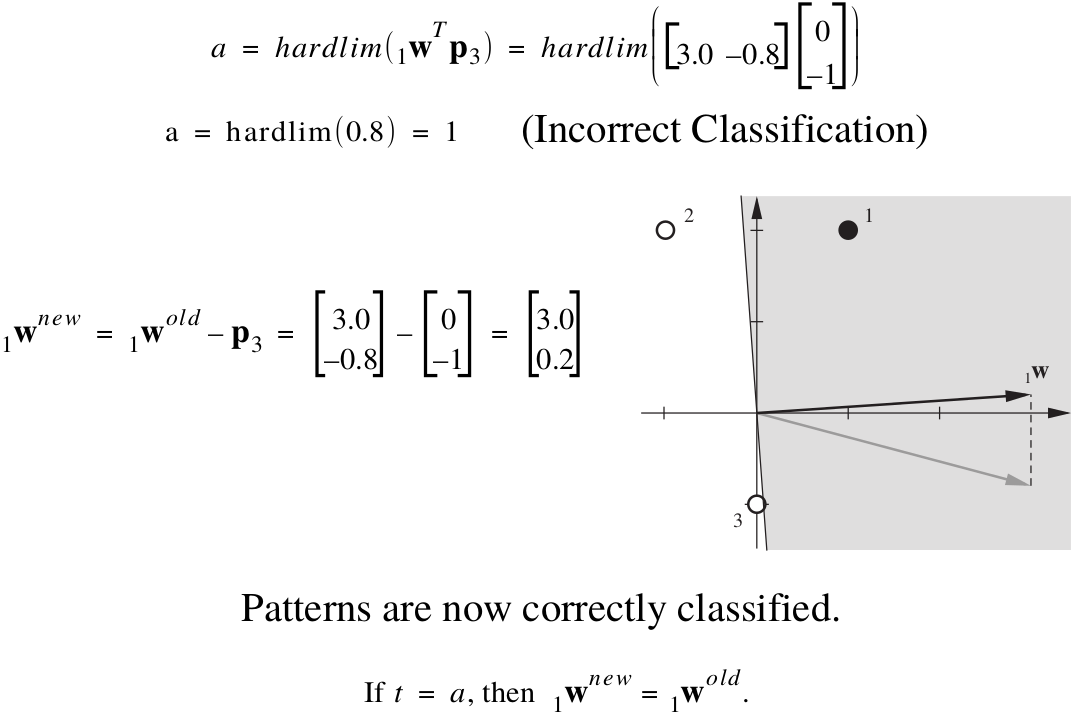
\includegraphics[width=.9\linewidth]{imgs/perceptron_ex_5}
  \end{figure}
\end{frame}

\begin{frame}
  \vspace{.5cm}
  \textbf{Unified Learning Rule}
  \begin{figure}
    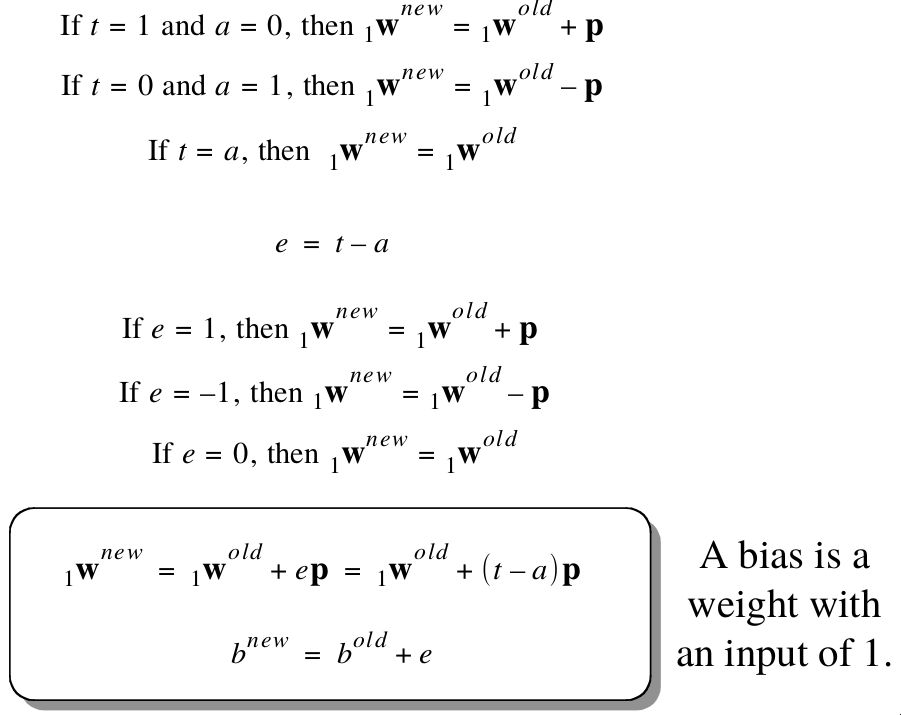
\includegraphics[width=.9\linewidth]{imgs/perceptron_ex_6}
  \end{figure}
\end{frame}

% \begin{frame}
% % $p_2 = -\frac{b}{w_{1,2}}$, if $p_1 = 0$ \qquad
% % $p_1 = -\frac{b}{w_{1,1}}$, if $p_2 = 0$
% \textbf{Perceptron's Learning Rule} \\ \hfill \break
% \centering
% If $t = 1$ and $\alpha = 0$, then $w^{new} = w^{old} + p$ \\
% If $t = 0$ and $\alpha = 1$, then $w^{new} = w^{old} - p$ \\
% If $t = \alpha$, then $w^{new} = w^{old}$ \\
%
% $$e = t - \alpha$$
% If $e = 1$, then $w^{new} = w^{old} + p$ \\
% If $e = -1$, then $w^{new} = w^{old} - p$ \\
% If $e = 0$, then $w^{new} = w^{old}$ \\ \hfill \break
%
% $w^{new} = w^{old} + ep = w^{old} + (t-\alpha)p$ \\
% $b^{new} = b^{old} + e$
%
% \end{frame}

\begin{frame}
  % \textbf{AND gate example} \\
  %
  % \[
  % p_1 =
  % \begin{bmatrix}
  %   0 \\
  %   0
  % \end{bmatrix}
  % , t_1 = 0
  % \quad
  % p2 =
  % \begin{bmatrix}
  %   0 \\
  %   1
  % \end{bmatrix}
  % , t_2 = 0 \quad
  % p_3 =
  % \begin{bmatrix}
  %   1 \\
  %   0
  % \end{bmatrix}
  % , t_3 = 0
  % \quad
  % p4 =
  % \begin{bmatrix}
  %   1 \\
  %   1
  % \end{bmatrix}
  % , t_4 = 1\]
  Linera regression learn the rules \\

  \textbf{Perceptron convergence theorem:} (link) \\
  The perceptron learning rule will converge to a weight vector (not necessarily unique) that  gives  the  correct  response  for  all  training  patterns,  and it will do so in a finite number of steps. \\
  Rosenblatt was so confident that the perceptron would lead to true AI, that in 1959 he remarked: \\
  \textit{[The perceptron is] the embryo of an electronic computer that [the Navy] expects will be able to walk, talk, see, write, reproduce itself and be conscious of its existence.}


  Python script - draw/update boundaries while learning!!! \\
  https://cs.stanford.edu/people/karpathy/convnetjs/demo/classify2d.html \\
  1 neuron demo - gates, function approximation (y = 2x), house prices, etc \\
(gradient descent)
\end{frame}


\begin{frame}

\vspace*{.5cm}
\textbf{Marvin Minsky and Seymor Papert - XOR problem [1969]} \\
Along with the double-PhD wielding Seymor Papert, Minksy wrote a book entitled Perceptrons that effectively killed the perceptron, ending embryonic idea of a neural net. They showed that the perceptron was incapable of learning the simple exclusive-or (XOR) function. Worse, they proved that it was theoretically impossible for it to learn such a function, no matter how long you let it train. Now this isn’t surprising to us, as the model implied by the perceptron is a linear one and the XOR function is nonlinear, but at the time this was enough to kill all research on neural nets \\

python demo - XOR problem (boundaries cant converge) \\
Linear model!!! meaning a straight line or a linear hyperplane


The First AI Winter (1969): brace yourselves - winter is coming

\end{frame}

\begin{frame}
Multi-Layer Perceptron (MLP) \\
Sigmoid activation function \\

All powered by BackProp [1986]!!! \\
Back Propagation 231n Stanford
\end{frame}

\begin{frame}
machine learning is all about a computer learning the patterns that distinguish things \\
map x to y example (y = x-1)
\end{frame}

\begin{frame}
  Laurence Moroney \\
traditional programming vs ML (rules + data = ans VS ans + data = rules) \\
the computer will figure out the rules \\
+ examples slides
\end{frame}

\begin{frame}
timeline (pic from thesis) - artificial neuron, perceptron, XOR problem, AI winter, back prop, MLP, AlexNet
\end{frame}

\end{document}
